\subsection{A Biblioteca FEniCS}

FEniCS é uma ferramenta computacional de código aberto que tem por objetivo a resolução de equações diferenciais parciais (EDPs). O FEniCS oferece rapidez para traduzir modelos físico-matemáticos em códigos de elementos finitos escritos nas linguagens de programação Python e C++ \cite{Fenics}. No programa estão implementadas a biblioteca fundamental  DOLFIN e outras funcionalidades especializadas. 

O DOLFIN fornece um ambiente de solução de problemas para modelos baseados em EDPs, incluindo estruturas de dados e algoritmos para malhas computacionais e abstrações de elementos finitos. O DOLFIN fornece classes para operar com matrizes, vetores, elementos diversos e espaços funcionais, entidades importantes para computação de elemento finitos. A interface foi projetada com o propósito de ser simples. Para resolver EDPs usando a interface DOLFIN, os usuários devem expressar os problemas na forma variacional usando a linguagem específica UFL \cite{Logg}. A Fig. \ref{fig:dolfin} exemplifica os componentes mais relevantes da biblioteca DOLFIN.
\begin{figure}[H]
	\centering
	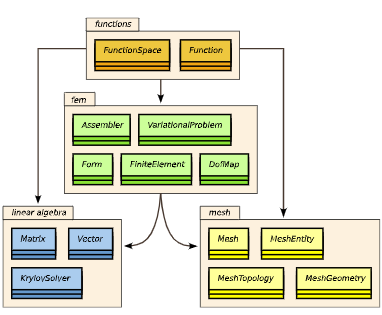
\includegraphics[scale=1]{img/esquema_dolfin.png}
	\caption[Componentes mais relevantes da biblioteca DOLFIN.]{Componentes mais relevantes da biblioteca DOLFIN \cite{Logg}.}
	\label{fig:dolfin}
\end{figure}